\section{Adding Partitioning to the CAD Flow}
\label{sec:CADflow}
TODO: Javeed

Given that the number of signals that can cross the interposer between FPGA dice is considerably more limited than within an FPGA, using a partitioner to divide the circuit into one partition per die is a promising CAD flow.

\subsection{CAD Flow Variations}
The overall CAD flow, including the partitioning steps, is shown in Figure \ref{fig:partitioning_cad_flow}.
\begin{figure}[!htbp]
\centering
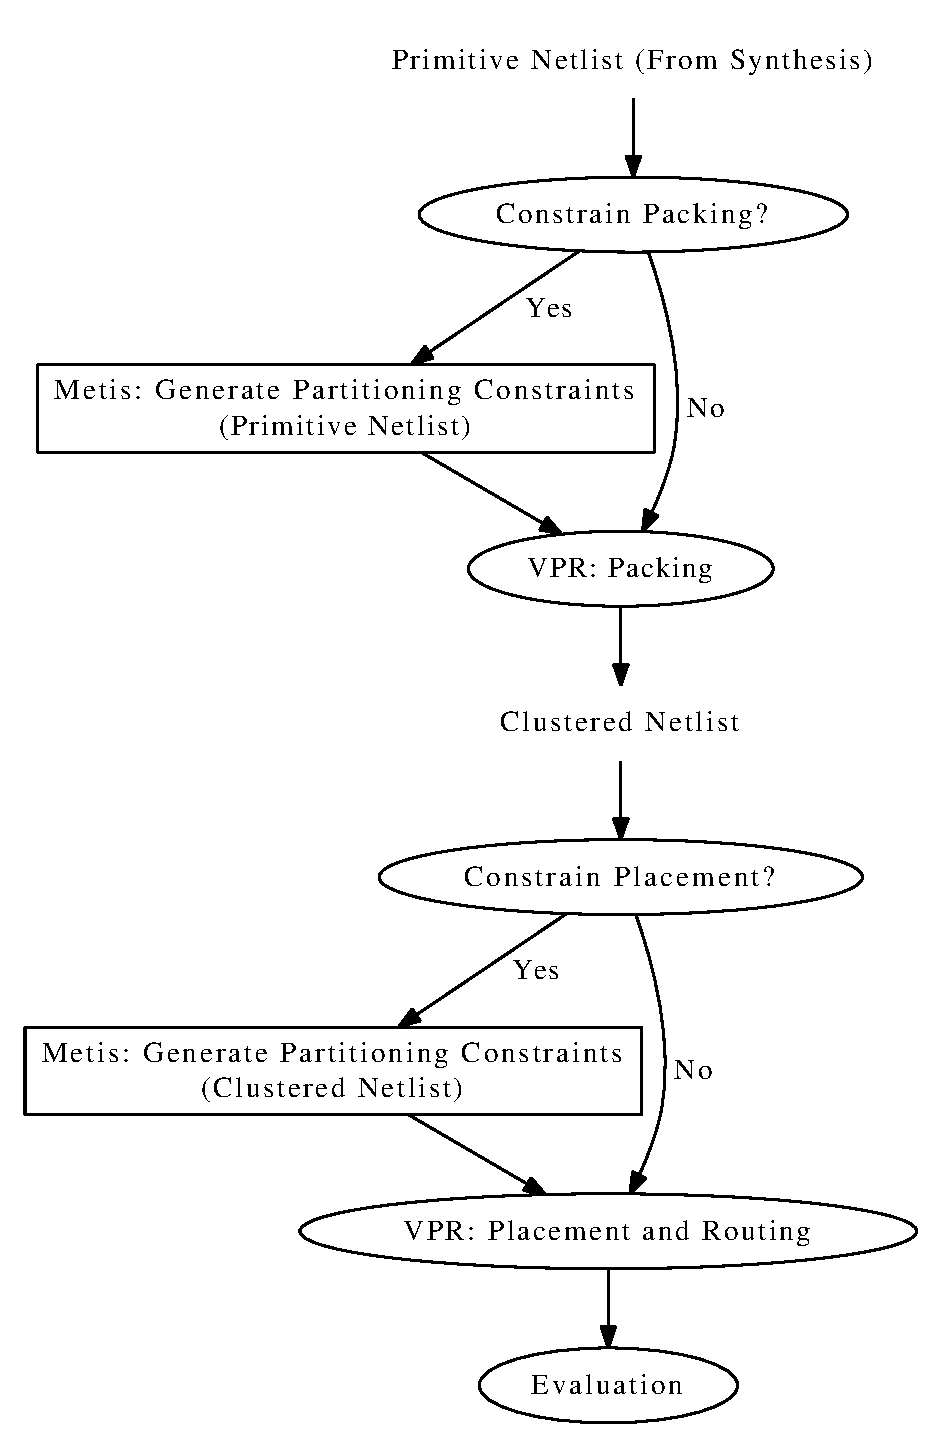
\includegraphics[width=\linewidth]{partitioning_cad_flow.eps}
\caption{Possible ways to add partitioning to the VPR CAD flow.}
\label{fig:partitioning_cad_flow}
\end{figure}

\subsubsection{Partitioner Stage}\label{sec:partitioner_stage}
As shown in Figure \ref{fig:partitioning_cad_flow}, we explore the effect of circuit partitioning at two different stages of the CAD flow. The first possibility is to partition the netlist of primitive elements (LUTs, FFs, RAM slices, etc.) before packing into the larger function blocks such as logic blocks and (32 kb) RAM blocks. In this flow the partitioning constraints must be respected by the packer; it must not pack two primitives assigned to different partitions (dice) into the same function block. We updated the VPR clustering algorithm to respect this new legality constraint.

The second possible way to incorporate partitioning is after packing, where partitioning is applied to the function block (cluster-level) netlist. Each partition is then assigned (randomly) to a separate FPGA die. The partitioning constraints must then be respected by the placer; it is free to move function blocks around within a die, but not across interposer cutlines. These two partitioning flow options can be combined -- if partitioning is applied before packing, one can to pass the partition information to the placement stage as well. The post-packing placement constraints can be derived from the primitive block partitioning, with the valid placement region for a given function block being equal to the intersection of the valid placement regions of the primitives packed into that function (clustered) block. There are, therefore, four possible partitioning flows:

\begin{enumerate}
  \item Leaving both the packer and the placer unconstrained. This is the base flow that does not use partitioning, as described in Section \ref{cadSection}.
  \item Partitioning the primitive netlist to guide the packer, leaving the placer unconstrained.
  \item Leaving the packer unconstrained, and partitioning the function block (clustered) netlist to guide the placer.
  \item Partitioning the primitive netlist to guide the packer, and constraining the placer based on constraints derived from partitioning, as described above.
\end{enumerate}

\subsubsection{Partitioning Tool}
Two well-known freely available graph partitioning tools are Metis~\cite{karypis1998multilevelmetis} and hMetis~\cite{karypis1999multilevelhmetis}. Metis operates on graphs, while hMetis operates on hypergraphs -- a hypergraph is a generalization of a graph, where each edge can connect any number of vertices. It is most natural to represent a circuit netlist as a hypergraph, where the vertices are netlist pins (or blocks) and the hyperedges are the nets joining the pins. Based on that criterion alone, hMetis is the most appropriate choice of partitioner. However, there are other issues to consider for the circuit netlist partitioning use case.

Graph partitioning algorithms generate partitions of a circuit while satisfying ``balance constraints''. The balance constraints exist to drive the algorithm away from the trivial partitioning solution where all vertices are in the same partition, leaving all other partitions empty. An example of a basic balance constraint is one which requires an equal number of vertices in each partition. Generally such a perfect balance overly restricts the solution, so some fractional ``unbalance'' is allowed; in this work we use $0.05$ ($5\%$). For two partitions, $P1$ and $P2$, this translates to $[ref Metis]$:

\begin{equation}\label{eq:balance_constraint}
\frac{|P1|}{|P1 \cup P2|} \in [0.5 - unbalance, 0.5 + unbalance]
\end{equation}

To derive an appropriate balance constraint for our use case, consider that FPGA circuit netlists may contain different block types such as LUTs, registers, RAM slices, and multipliers, among others. The basic balance constraint of (\ref{eq:balance_constraint}), applied to the two partition case with only LUTs and multipliers would ensure that the total block count (sum of the LUT count + multiplier count) in each partition is roughly balanced.

In our architecture, each FPGA die is identical, and therefore each die has the same number of resources as every other die. However, the number of available instances of each block type is not equal -- there are usually more LUTs than multipliers, for example. The problem with the simple balance constraint in the case of multiple block types is that the capacity of each partition is not taken into account on a per-block-type basis. It is therefore possible to generate partitions that cannot be realized because the number of resources of each type is not balanced across partitions, even though the total number of resources is balanced. For example, there is nothing preventing the partitioner from moving all LUTs to partition 1 and all multipliers to partition 2, which would not be physically realizable because partition 1 may not have enough LUTs to implement the desired partitioning (and the LUTs in partition 2 would be completely unused.) A technique is to enforce a balance constraint on each type of block, $i$:

\begin{equation}
\forall i, \abs*{ \frac{| P1_i |}{|P1_i \cup P2_i |} - 0.5} < unbalance
\end{equation}
where $P1_i$ denotes the set of all blocks of type $i$ in partition 1.

We refer to this type of per-block set of constraints as heterogeneous balance constraints. Note that there are complex legality constraints governing which LUTs and FFs can be packed into legal logic blocks, as well as which multipliers can be packed into legal DSP blocks [ref AAPack]. As the partitioner is not aware of these constraints, flow 3 above (which runs the partitioner after function block packing) will be able to more precisely balance resource use across partitions.

The latest public version of hMetis does not support heterogeneous balance constraints, thourgh Metis does. Metis was used in our CAD flow. However, as discussed earlier, the circuit netlist is most naturally represented as a hypergraph, and so it needs to be transformed to a graph before Metis can process it.

\subsubsection{Hypergraph to Graph Transformation}\label{sec:hypergraph_to_graph}
We transformed the circuit netlist hypergraph to a graph in the following way:
\begin{enumerate}
\item For each hyperedge of the circuit netlist hypergraph, we generated a graph (the \emph{per-net subgraph}).
\item We combined all of the per-net subgraphs, summing the edge weights for edges appearing in more than one per-net subgraph, to generate the total netlist graph.
\end{enumerate}

We explored several ways to generate the per-net subgraphs. The two parameters in this operation are the graph topology and the edge weight scheme. We considered two subgraph topologies, clique and star, as illustrated in Figure \ref{fig:star_clique}.

\begin{figure}[!htbp]
\centering
\subfigure[]{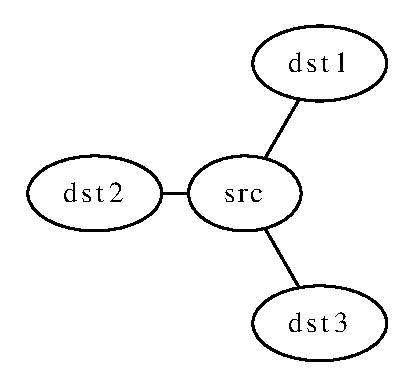
\includegraphics[width=0.45\linewidth]{star.eps}}
\subfigure[]{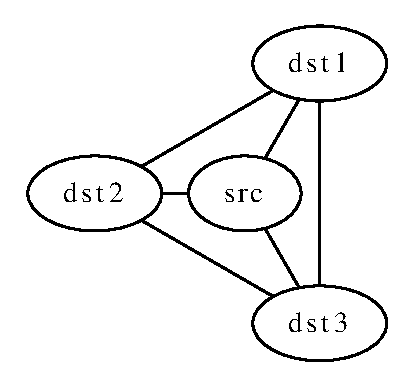
\includegraphics[width=0.45\linewidth]{clique.eps}}
\caption{(a) Star and (b) clique graph topologies.}
\label{fig:star_clique}
\end{figure}

We assigned the same edge weight to every edge of the generated subgraph. Edge weights were computed based on the number of vertices in the hyperedge, $n$, and we considered edge weights equal to $1$, $1/n$, and $1/n^2$. Note that the vertices in the generated total netlist graph are the same as the vertices in the original circuit netlist hypergraph.

Figure \ref{fig:hyperedge_to_graph} shows how a netlist of three blocks and two nets is transformed into its component subgraphs.

\begin{figure}[!htbp]
\centering
\subfigure[]{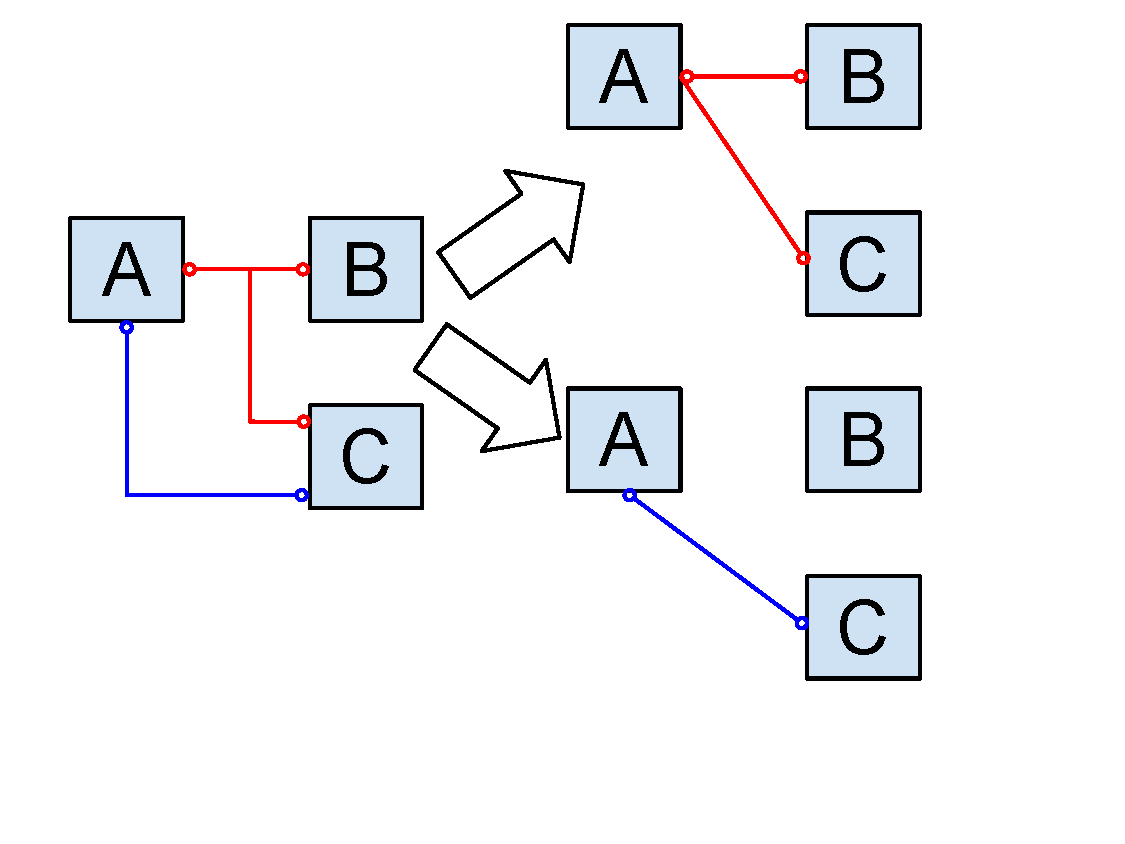
\includegraphics[width=0.45\linewidth]{hg2g_star.pdf}}
\subfigure[]{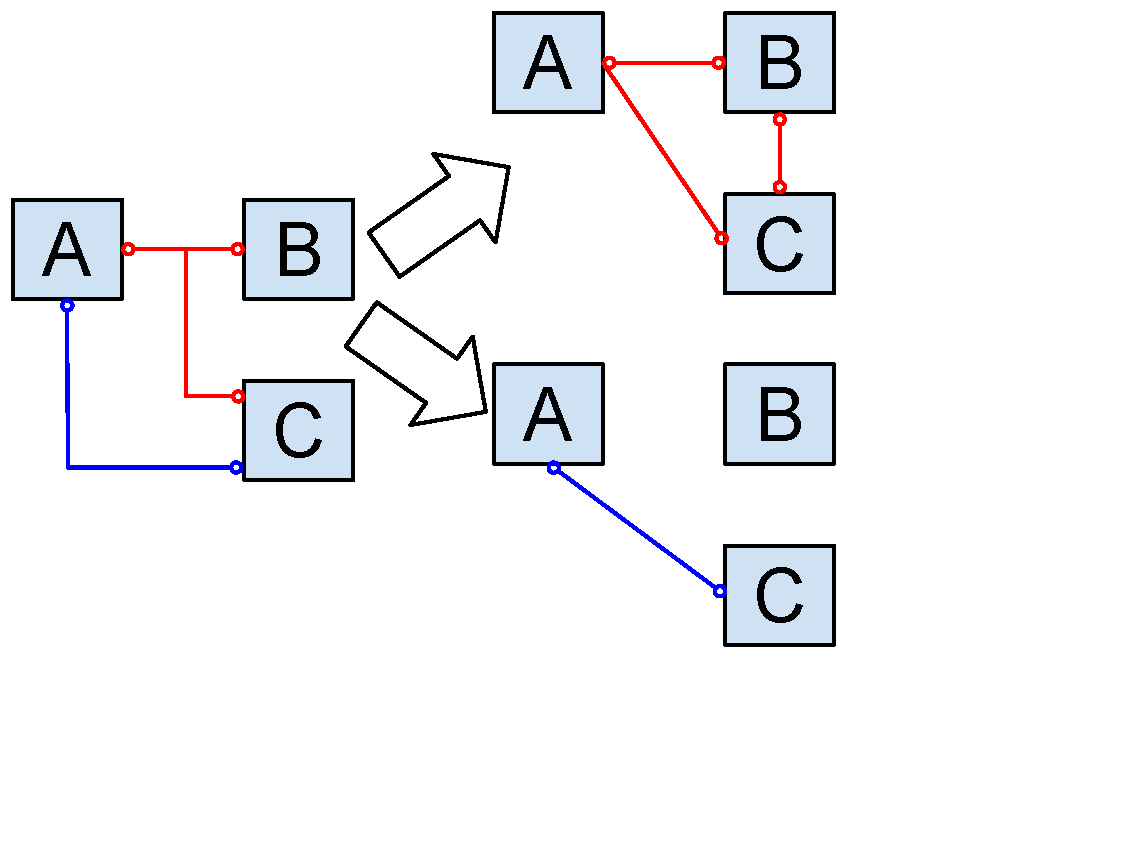
\includegraphics[width=0.45\linewidth]{hg2g_clique.pdf}}
\caption{The hypergraph to graph transformation with (a) the star topology, and (b) the clique topology.}
\label{fig:hyperedge_to_graph}
\end{figure}

The parameters of graph topology and edge weight were evaluated by generating the total primitive netlist graph and running it through the Metis partitioner to generate two partitions. The results of the different schemes were ranked based on the hyperedge cutsize, which is the number of hyperedges crossing the cutline, as illustrated in Figure ??. The hyperedge cutsize is a proxy for the routability of the circuit, as the cutsize is the number of nets that cross the interposer boundary. To compute the hyperedge cutsize, we applied the partitioning result (which assigns each vertex to a partition number) to the original untransformed hypergraph, and counted the number of hyperedges whose vertices were spread across different partitions. We computed the hyperedge cutsize for every combination of graph topology and graph edge weight scheme, across several circuits. The results are shown in Figure \ref{fig:graph_topology_cutsize}.

\begin{figure}[!htbp]
\centering
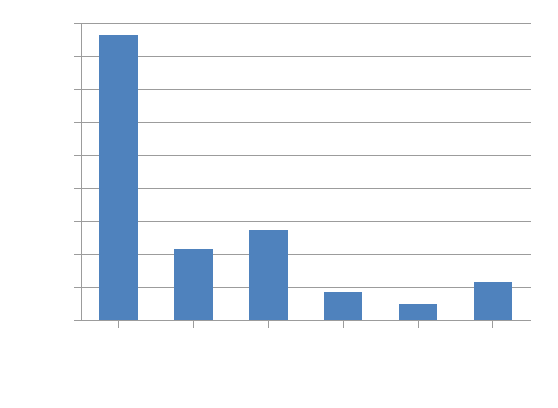
\includegraphics[width=\linewidth]{graph_topology_cutsize.eps}
\caption{Hypergraph cut size achieved by Metis with different hyperedge models and weightings. n is the number of vertices on a hyperedge.}
\label{fig:graph_topology_cutsize}
\end{figure}

The performance of the clique topology is significantly worse than that of the star topology, regardless of edge weight scheme. An intuitive explanation for this result is that with the clique topology, the partitioner does not have knowledge of which vertex is the source of a net and which vertices are sinks. In contrast, the star topology clearly differentiates sources from sinks and this appears to give the partitioner an “anchor point” that pulls all hyperedge fanouts toward the source. Additionally, if $n$ is the average number of vertices in a hyperedge, the clique topology generates $O(n^2)$ edges while the star topology generates only $O(n)$ edges, so the star topology saves both memory and runtime.

For both topologies, the $1/n$ edge weight scheme gives the smallest cut size on average. This can be explained intuitively in terms of the total edge weight over all edges of the graph. The star $1$ (constant) edge weight scheme assigns a total weight of $n$ to each net, which heavily weights high-fanout nets. In contrast, the star $1/n$ scheme assigns the same total weight of $1$ to each net. The star $1/n^2$ scheme penalizes high-fanout nets relative to lower-fanout nets. Since we seek to minimize the hyperedge cut, it makes intuitive sense to weight all hyperedges equally, and the star $1/n$ scheme achieves this.

To validate the choice of hyperedge cutsize as a proxy for circuit routability, we ran the partitioning CAD flow for each graph topology and edge weight scheme, across several circuits. We use an unbalance of $5\%$, split the clustered netlist into two partitions (constraining only the placer), cut $80\%$ of the wires crossing the interposer, and impose a $1ns$ delay penalty for wires crossing the interposer. To accommodate unbalance in the placement engine, we increase the size of the grid of complex blocks that make up the FPGA device. Relative to the minimum device size required for placement (without partitioning constraints), we add $10\%$ to the complex block grid width and $10\%$ to the grid height. Figure \ref{fig:graph_topology_mcw} shows the geometric mean of the minimum channel width required for a successful route, for each of the graph topology and edge weight combinations.

\begin{figure}[!htbp]
\centering
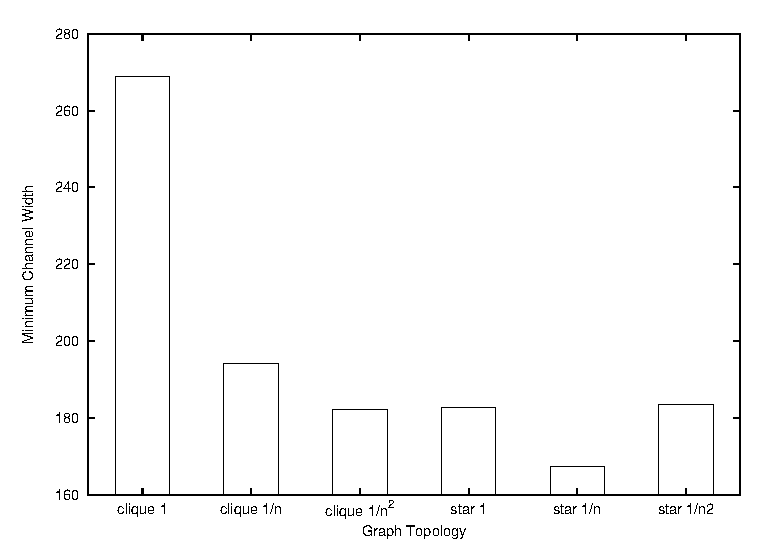
\includegraphics[width=\linewidth]{graph_topology_mcw.eps}
\caption{Minimum channel width achieved by VPR with different hyperedge models and weightings. n is the number of vertices on a hyperedge.}
\label{fig:graph_topology_mcw}
\end{figure}

The star topology with 1/n edge weights achieves the best minimum channel width, confirming that hyperedge cutsize is a good proxy for routability. Consequently, we use this scheme in all future results in this paper. Unlike routability, we found that the post-routing critical path delay was not strongly impacted by the hypergraph conversion scheme used.

\subsubsection{Partitioner Stage Results}\label{sec:partitioner_stage_results}
We compare the performance of the four CAD flow variations described in Section \ref{sec:partitioner_stage} on the 8 largest VTR benchmarks. We again use an unbalance of $5\%$ and split the clustered netlist into two partitions (constraining the packer and/or the placer, as required by the flow under test). The interposer parameters (\% wires cut = $80\%$ and delay increase = 1 ns) and bloat factor ($10\%$ in each dimension) are the same as in Section \ref{sec:hypergraph_to_graph}. Figure \ref{fig:flows_mcw} shows the minimum routable channel width for each partitioning CAD flow variation.

\begin{figure}[!htbp]
\centering
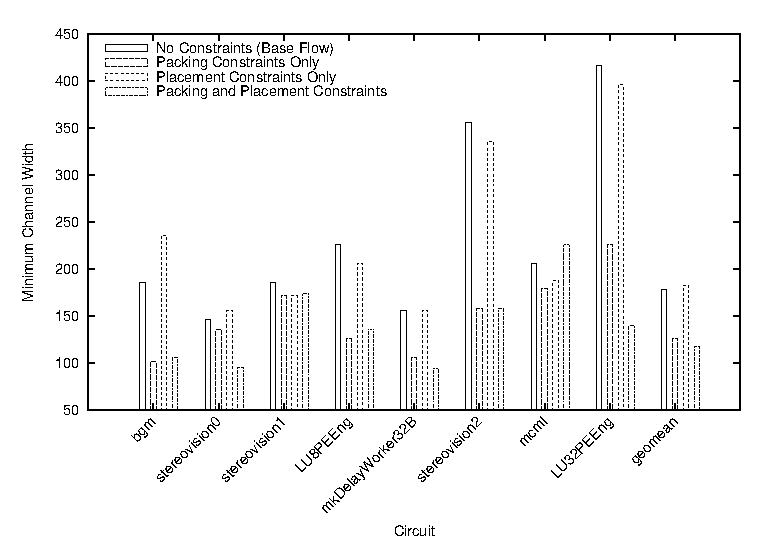
\includegraphics[width=\linewidth]{vpr_flows_mcw.eps}
\caption{Minimum channel width achieved by VPR with the different partitioning flows.}
\label{fig:flows_mcw}
\end{figure}

On average, the best minimum channel width was obtained when constraining both packing and placement. However, constraining packing alone performed significantly better than constraining placement alone. This shows that the VPR packer strongly benefits from partitioning constraints when targeting an interposer-based architecture, likely because it forbids the packing of primitives that are not naturally related into one function block. Interestingly, other recent work targeting conventional FPGAs has shown that using a partitioner to guide packing benefits routability [Wenyi Feng, et al, “Rent’s Rule Based Packing for Routability Optimization,” FPGA 2014 ]. On the other hand, The VPR placement algorithm with the enhancements described in Section 4 sees only a modest routability benefit from the partitioning constraints.

For the same set of circuits, we computed the critical path delay at a channel width equal to 1.3x the minimum. The results are shown in Figure \ref{fig:flows_crit_path}.

\begin{figure}[!htbp]
\centering
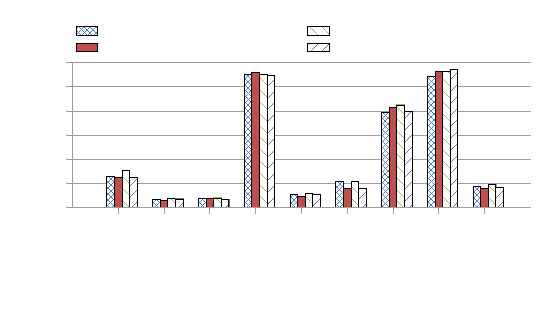
\includegraphics[width=\linewidth]{vpr_flows_crit_path.eps}
\caption{Critical path delay achieved by VPR with the different partitioning flows.}
\label{fig:flows_crit_path}
\end{figure}

On average, the critical path delay did not vary significantly between the different partitioning CAD flows, but it appears that partitioning before packing may slightly improve circuit speed, while enforcing these partitioning constraints during placement may slightly reduce circuit speed.

Considering both routability and delay, the best CAD flow constrained both packing and placement with the partitioning result and this is the flow we use in the remainder of this paper.

\subsubsection{\% wires cut}
To see how well the CAD flow works for a range of interposer architectures, we varied the fraction of wires cut and measured the average minimum channel width over the 8 largest VTR circuits. As shown in Figure \ref{fig:wires_cut}, this new flow is a significant improvement over that of [] for FPGAs where more than half the wires are cut at interposer boundaries. It is slightly worse than the traditionally FPGA CAD flow even for an architecture with 0\% of the wires cut, which is a monolithic FPGA, presumably because we have restricted the placer's freedom.

\begin{figure}[!htbp]
\centering
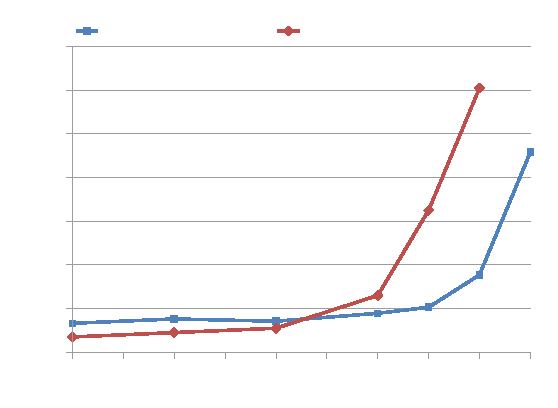
\includegraphics[width=\linewidth]{wires_cut.eps}
\caption{Impact of partitioning-based CAD flow on routability for a range of architectures.}
\label{fig:wires_cut}
\end{figure}

\subsubsection{Bloating of the Clustered Netlist due to Partitioning Constraints}
The additional constraints on the packer imposed by partitioning may result in a less dense packing. Figure \ref{fig:packing_bloat} compares the number of complex blocks in the partitioning-constrained and unconstrained clustered netlists.

\begin{figure}[!htbp]
\centering
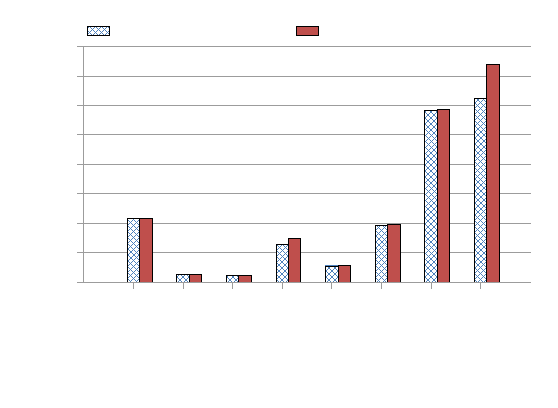
\includegraphics[width=\linewidth]{packing_bloat.eps}
\caption{Packing bloat.}
\label{fig:packing_bloat}
\end{figure}

On average, the packing-constrained netlist contained $3.2\%$ more complex blocks than the unconstrained netlist. The LU8PEEng and LU32PEEng circuits were the most affected by this packing bloat. In those circuits, we found that the packing bloat was due almost entirely to poor packing of memory blocks; an interesting area for future work would be to augment the partitioner to understand that some RAM primitives are best kept together in one partition.
